\documentclass[a4paper]{article}

\usepackage{amssymb,,hyperref,graphicx}

\title{Assignment 4 - Question 5}
\author{Ory Band \texttt{300479425}}
\date{\today}

\newtheorem{thm}{Theorem}

\usepackage{fancyhdr}
\pagestyle{fancy}
\lhead{Ory Band \texttt{300479425}}
\rhead{}
\renewcommand{\headrulewidth}{0.4pt}
\renewcommand{\footrulewidth}{0.4pt}

\begin{document}

\section {Question 5 - AdaBoost vs. SVM}

Dataset URL: \url{https://archive.ics.uci.edu/ml/datasets/Skin+Segmentation}
\\\\
Using the same dataset from the last assignment (Skin segmentation),
I tested AdaBoost on varying iterations ranging from 1 to 200.
I used linear threshold decision stumps as weak classifiers.
\\\\
The success rate was high on all iteration runs,
but showed notable improvement when running more than 100 iterations.
The higher success rates were consistent around 96\% success.
\\\\\
Since the dataset is pretty much seperable,
SVM also showed a good success rate of 92.65\%.
\\\\
I suspect the difference in the error between the two learners
is due to the weak classifiers (decision stumps) in use,
which produce a more precise classifier "polygon" (function).
In comparison, SVM produces a linear classifier which isn't as "precise".

\begin{figure}[h!]
    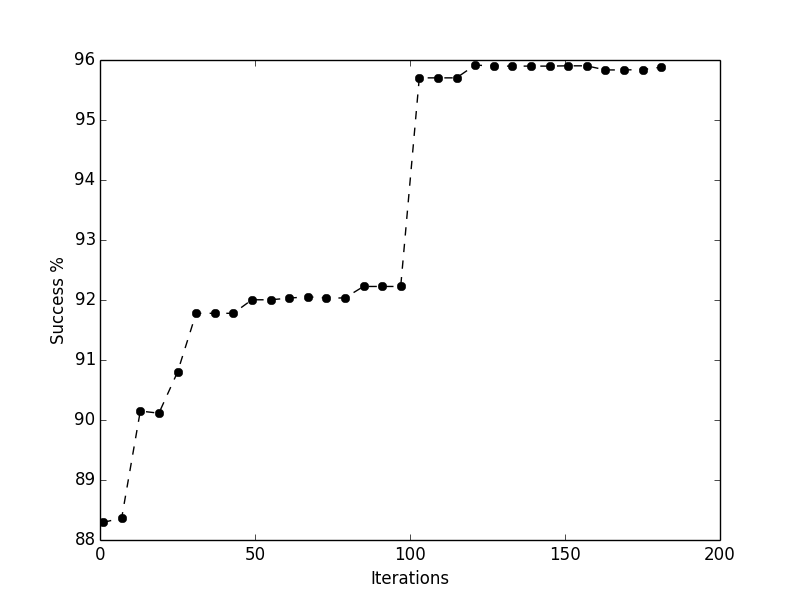
\includegraphics[width=1\textwidth]{adaboost_iterations.png}
\end{figure}

\end{document}
